% 3rd - Recognition
%% Includes: Alignment methods, matching, descriptors, hypothesis verification

\chapter{Sparse feature matching}
\label{cha:feature}

Solutions to problem stated in section \ref{sec:problem} are commonly divided \cite{something} into feature-based and template-based. The former approach, also referred to as local matching, is focused on comparing point neighbourhoods between the scene and model datasets. 

The solution in such methods is composed of several steps. Firstly, an input subset with elements of rich and distinguishable neighbourhood information is selected. Points that belong to this subset are referred to as \textit{keypoints}. For each keypoint, its neighbourhood information is expressed in the form of a \textit{descriptor} vector. By the means of selected metric, commonly the $L_2$ norm, descriptors are further compared between the scene and model datasets, to find \textit{correspondences} with minimal distance. Such point pairs are then grouped to share similar geometric constrains and finally, the largest clusters are used to calculate affine transformation, which renders the initial problem solution.

The inherent locality of feature matching methods has direct implications on the solution performance. Such methods are by design robust to occlusions \cite{something}. Each point is processed independently, which enables data parallelization to boost time performance. Conversely, keypoint identification requires costly analysis of the whole input dataset, thus a balance between the recognition performance and time effectiveness is required \cite{somethin} for real-time applications.

%---------------------------------------------------------------------------

\section{Shape description} %SHOT}
\label{sec:shape} %shot}

There is a multitude of proposals for shape key-point detectors existing in literature. An overview and performance evaluation of the most popular methods can be found in \cite{keypoints1} and \cite{keypoints2}. From both evaluations, the \textit{Intrinsic Shape Signatures} (ISS) \cite{ISS} detecor is worth particular attention. \cite{keypoints1} states that ISS, as a fixed-scale detector, copes well with full three-dimensional models and provides a proper balance between the repeatability rate and time efficiency. In \cite{keypoints2}, the ISS is evaluated with the best repeatability rate among detector implementations available in PCL. The ISS introduces a saliency measure, defined by the smallest eigenvalue of the neighbourhood scatter matrix. For a given point $p$ and its neighbourhood $N$, the scatter matrix $\Sigma$ is given by
\begin{equation}
\label{eq:scatter}
\Sigma(p,N) = \frac{1}{|N|} \sum\limits_{q\in N}(q -\mu_p)(q - \mu_p)^T,\ \mu_p = \frac{1}{|N|}\sum\limits_{q\in N}q
\end{equation}
% originally defined as weighted matrix, need to check how its implemented
By denoting the eigenvalues of $\Sigma(p, N)$ as $\lambda_1 > \lambda_2 > \lambda_3$, the ISS detector classifies $p$ as a keypoint, if the following condition is satisfied
\begin{equation}
\label{iss}
\frac{\lambda_2}{\lambda_1} < \epsilon_1 \  \land \  \frac{\lambda_3}{\lambda_2} < \epsilon_2 \ \land \  \lambda_3 > \epsilon_3.
\end{equation} 
Thresholds $\epsilon_1$ and $\epsilon_2$ are meant to provide sufficient difference between variations along each principal direction, which aids in estimation of a repeatable reference frames for further description stages. The third threshold $\epsilon_3$ ensures that the variations are large enough to consider the point as interesting. A further improvement to the ISS detection criteria is to apply non-maximum suppression over the saliency measure computed at each point. With this edge thinning technique, a point is classified as a keypoint, if it has the largest $l_3$ over its neighbourhood.  An example of keypoints detected with ISS is presented on figure \ref{fig:iss}. The object (cleaning spray in the center of the figure) has marked points in areas of rich shape information, like the bottleneck or the nozzle. It is also visible, that ISS classifies wrong points in two cases. Firstly, when a point lies on a visibility boundary (i.e. the edges of flat surfaces in the figure), thus it should be extended with boundary detection as described in xx. Secondly, when the sensor noise is high (distant wall flat surface in upper left edge of the figure). This issue can be handled by ignoring points above certain z-distance from the sensor or by adaptatively selecting neighbourhood radius for saliency measure.
%select rich shape object from willow = 13
%implement hardload and iss, measure avg time
%implement in cuda

\begin{figure}[h]
\centering
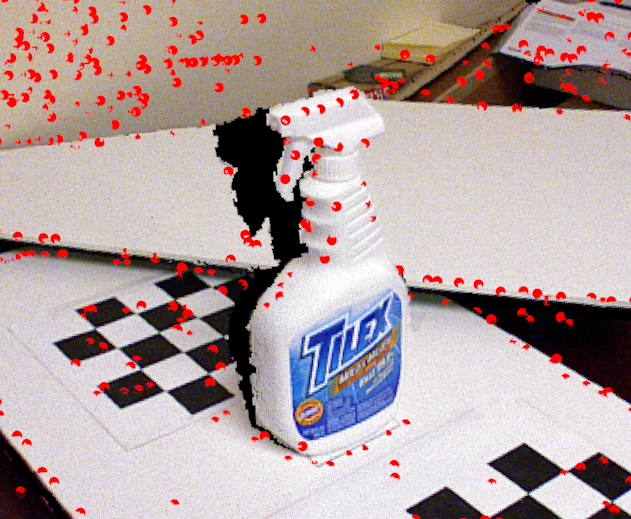
\includegraphics[width=0.8\textwidth]{fig/ISS}
\caption{ISS keypoints (marked with red) computed with $\epsilon_1 =  \epsilon_2 = 0.75$ and $\epsilon_3 = 0.0005$ }
\label{fig:iss}
\end{figure}

The overall time complexity of ISS classification is at the order of $O(nk)$, where $n$ is the image size and $k$ is the max neighbourhood size. This translates into average execution times on target platforms, provided in table \ref{tab:issexec}.

\begin{table}[h]
\centering
\begin{tabular}{r || c | c}
& NVidia Jetson TK1 & Lenovo Y50-70 \\
 \hline
 \hline
 PCL ISS& 4s & 4s \\
 PCL ISSBD& 4s &  4s \\
 CUDA ISS& 4s & 4s \\
 CUDA ISSBD& 4s & 4s
\end{tabular}
\caption{ISS detector time performance statistics.}
\label{tab:issexec}
\end{table}

It is important to note, that in practical applications the keypoint detection step is often replaced by volumetric down sampling. About voxel grid. Model is densely grained. This avoids computational costs of keypoint detection, but increases the complexity of further matching and clustering stages. How to choose this tradeoff.
%In \cite{keypoints-learning}, authors propose a random-forest classifier to be trained for detection of the best interest points for any chosen descriptor.

%Provide complexity, measure time perf (and invariance to transformations?). Can be skipped with uniform.

Descriptor comparison. Take SHOT \cite{SHOT}. Complexity, time perf. Extension with color. \cite{CSHOT}

%----------------------------	-----------------------------------------------

\section{Texture description} %ORB}
\label{sec:colour} %orb}

matching \cite{ORB}

%---------------------------------------------------------------------------

\section{Clustering}
\label{sec:clustering}

geometric consistency, hough

%---------------------------------------------------------------------------

\section{Alignment}
\label{sec:alignment}

umeyama, ransac

